\documentclass[11pt,a4paper]{report}
%\fontfamily{cmss}
\hfuzz=9999pt % "fix" hbox overfull
%Path relative to the .tex file containing the \includegraphics command
\usepackage{graphicx}
\usepackage{hyperref}
\hypersetup{
    colorlinks=true,
    linkcolor=blue,
    filecolor=magenta,      
    urlcolor=blue
}

\begin{titlepage}
\title{BU5526 - Portfolio Analysis \\ Lecture Notes}
\author{Rodrigo Miguel}
\date{\today}
\end{titlepage}



\begin{document}
\maketitle
\tableofcontents

\chapter{Introduction}
\section{Asset Pricing}
\subsection{Asset}
Something valuable that an entity owns, benefits from, or has use of, in generating income.
\subsection{Asset Pricing}
Needed to buy/sell at a fair price.
\begin{itemize}
    \item Obtained by discovery process:
        \begin{itemize}
            \item Demand and supply forces.
        \end{itemize}
    \item The price of an asset is simply the current value of its cash-flows.
    \[ PV = \frac{FV_1}{(1+r)^1} + \frac{FV_2}{(1+r)^2}+ ... + \frac{FV_n}{(1+r)^n} \]
        \item What we need:
        \begin{itemize}
            \item Prediction of cash flows;
            \item Discount rate.
        \end{itemize}
\end{itemize}

\subsection{How to price a stock:}
\begin{itemize}
    \item Dividend Discount Model;
    \item FCF Model;
    \item Multipliers and Comparable approach.
\end{itemize}
Being able to estimate the required \textbf{rate of return} is everything you need to calculate the \textbf{value of any asset} - once you have predicted \textbf{future cash-flows}, including:
\begin{itemize}
    \item Estimating the value of a stock;
    \item Estimating the value of a firm.
\end{itemize}

\section{Portfolio Management}
\textbf{Prudent} administration of \textbf{investable} (liquid) assets, aimed at achieving an \textbf{optimum risk-reward ratio}.

\section{Mathematical Concepts}
\subsection{Mean} An average of different observations.
\begin{itemize}
    \item Useful to describe a population;
    \item \textbf{Arithmetical}: sum of observations divided by the number of observations (if with equal weights).
    \[\overline{X} = \frac{X_1 + X_2 + ... + X_n}{n}\]
    or
    \[\overline{X} = W_1 \times X_1 + W_2 \times X_2 + ... + W_n \times X_n\]
    \item \textbf{Geometrical}: n root of the product of observations.
    \[\overline{X}_G = \sqrt[n]{X_1 \times X_2 \times ... \times X_n}\]
    or
    \[\overline{X}_G = \sqrt[n]{X_1^{W_1} \times X_2^{W_2} \times ... \times X_n^{W_n}} \]
\end{itemize}
There is a reason to use arithmetical or geometrical mean.
\begin{itemize}
    \item \textbf{Equally weighted}: when all the observations have the same importance.
    \item \textbf{Unequally weighted}: different importance for different observations.
\end{itemize}

\subsection{Variance} Seen as an extension of the mean.
\begin{itemize}
    \item Dispersion to the mean (higher/lower):
    \begin{itemize}
        \item Average of differences from the mean.
        \[\sigma_x^2 = \frac{(X_1 - \mu_X)^2 + (X_2 - \mu_X)^2 + ... + (X_n - \mu_X)^2}{n}\]
    \end{itemize}
    
\end{itemize}

\subsection{Important Statistical Concept}
\begin{itemize}
    \item The formula is correct if we possess all the data on the population;
    \item If we only have a sample, we need to reflect "impreciseness" by removing "one degree of freedom".
    \[\sigma_x^2 = \frac{(X_1 - \mu_X)^2 + (X_2 - \mu_X)^2 + ... + (X_n - \mu_X)^2}{n-1}\]
\end{itemize}
This will \textbf{always} be the case in finance.

\subsection{Standard Deviation}
\[\sigma_X = \sqrt[2]{\frac{(X_1 - \mu_n)^2 + (X_2 - \mu_n)^2 + ... + (X_n - \mu_n)^2}{(n-1)}} \]

\subsection{Skewness}
Brings back the sign. A positive skewness means more positive-value and reversely.
\[\sigma_X^3 = \frac{(X_1 - \mu_n)^3 + (X_2 - \mu_n)^3 + ... + (X_n - \mu_n)^3}{n} \]

\subsection{Kurtosis}
Outweighs extremes - dropping the sign.
\[\sigma_X^4 = \frac{(X_1 - \mu_n)^4 + (X_2 - \mu_n)^4 + ... + (X_n - \mu_n)^4}{n} \]
A large Kurtosis means a lot of extreme values.
\begin{itemize}
    \item To get a \textbf{meaningful estimate:} \textbf{excess} kurtosis needs to be provided.
    \item Kurtosis of a normal distribution is 3.
\end{itemize}

\paragraph{Note:} Unbiased equations of these two indicators are slightly more complex, but computer packages provide them automatically.

\section{Assumptions of Mean-Variance Analysis}
\begin{itemize}
    \item Allows describing different assets simply.
    \item Assumes returns are normally distributed.
\end{itemize}
\subsection{Normal distribution}
\begin{itemize}
    \item Its mean and median are equal;
    \item It's defined by two parameters, mean and variance;
    \item It's defined around its mean with:
    \begin{itemize}
        \item 68\% of observations within $\pm$ 1$\sigma$ of the mean.
        \item 95\% of observations within $\pm$ 2$\sigma$ of the mean.
        \item 99\% of observations within $\pm$ 3$\sigma$ of the mean
    \end{itemize}
    \item Returns are not normally distributed.
    \begin{itemize}
        \item Skewed: not symmetric around the mean.
        \item Characterized by high probability of extreme event.
    \end{itemize}
\end{itemize}

\section{Returns on Financial Assets}
\subsection{Holding period return} Return from holding an asset for a specific period of time.
\[R = \frac{P_t - P_{t-1}}{P_{t-1}} + \frac{D_t}{P_{t-1}}\]
Capital gain + Dividend yield \\
Holding period returns = compound returns
\[R = [(1 + r_1) \times (1 + r_2) \times (1+r_3)] - 1 \]

\subsection{Geometric Mean Return}
\[\overline{R} = \sqrt[T]{(1+r_{i_1}) \times (1+r_{i_2}) \times ... \times (1+r_{i_T})} - 1\]
\subsection{Annualized Return} These returns should be capitalized.
\begin{itemize}
    \item Such as:
    \[ r_{annual} = (1+r_{period})^C - 1\] with C being the number of periods in a year.
\end{itemize}

\subsection{Portfolio Return}
\begin{itemize}
    \item When several assets are combined into a portfolio, we can compute the portfolio return.
    \item Weighted average of the returns of individual assets
    \[ R_p = W_1 \times R_1 + W_2 \times R_2\]
\end{itemize}

\subsection{Historical and Expected Returns}
\begin{itemize}
    \item Computed from historical data.
    \item What the investor expects to earn.
    \item Historical returns are different from expected returns.
\end{itemize}

\subsection{Ways of Calculating Expected Returns}
\begin{itemize}
    \item Gut feeling;
    \item Modelling - calculated from a formula.
\end{itemize}

\subsection{Standard deviation - Volatility}
\begin{itemize}
    \item Historical standard deviation;
    \item Defined as \textbf{risk} of equity return.
\end{itemize}

\subsection{Portfolio Variance}
\begin{itemize}
    \item Cannot simply add up two variances.
    \item Covariance:
    \[cov(X,Y) = E(XY) - E(X) \times E(Y)\]
    \begin{itemize}
        \item The more the two assets move in the same way, the higher the covariance.
        \item A negative covariance means the assets move in opposite directions.
    \end{itemize}
    \item Variance:
    \[ \sigma_v^2 = wCw^T \]
\end{itemize}

\subsection{Correlation and Portfolio Risk}
The correlation among assets determine the portfolio's risk.
\begin{itemize}
    \item Is a measure of tendency for N investments to act similarly;
    \item Can range from $-$1 and $+$1.
    \[\rho_{ij} = \frac{cov(R_i,R_j)}{\sigma_i \sigma_j}\]
\end{itemize}

\chapter{The Optimal Portfolio}
\section{Portfolio}
\subsection{The Portfolio Perspective on Investing}
One of the biggest challenges faced by individuals and institutions is to decide on how to invest for future needs. Should they invest in individual securities, or should they take a portfolio approach?
\\A portfolio and evaluating individual securities in relation to their contribution to the investment characteristics is important to achieve a "good" and "safe" return.
\subsection{Diversification: Avoiding Disaster}
Portfolio diversification helps investors avoiding disasters. It is of our utmost priority to balance investment weights as a way of having a good risk-return ratio.
\\On the other hand, it does not mean that, by reducing risk the portfolio will have reduced profits.
\begin{itemize}
    \item The portfolio approach provides investors with \underline{a way to reduce the risk} associated with their investment.
    \item Investors can choose the risk-return trade-off they prefer.
    \item A lower risk does not necessarily mean lower profits.
\end{itemize}
\subsection{Reducing Risk}
A Portfolio generally offers equivalent expected returns with lower overall volatility.
\\How to calculate its standard deviation?
\begin{itemize}
    \item An interesting feature of combining assets is that:
    \item \begin{itemize}
        \item While the combined return is the weighted average of individual returns, the combined variance is impacted by the covariance between securities.
    \end{itemize}
    \item{Covariance is how securities move together.}
\end{itemize}
\subsubsection{Variance of a Portfolio}
\[\sigma_p{^2} = wCw^T\]
or
\[\mu_v = w_1\mu_1 + w_2\mu_2\]
\subsubsection{Standard Deviation}
\[\sigma_p = \sqrt{\sigma_p{^2}}\]
or
\[\sigma_v{^2} = w_1{^2}\sigma_1{^2} + w_2{^2}\sigma_2{^2} + 2w_1w_2c_{12}\]
Remember that using correlation instead of variance, we can reformulate the variance equation:
\[\sigma_v{^2} = w_1{^2}\sigma_1{^2} + w_2{^2}\sigma_2{^2} + 2w_1w_2\sigma_1\sigma_2\rho_{12}\]

This equation shows that as long as $\rho_{12} is < 1$ adding more assets will reduce the overall variance of the portfolio.

\subsection{Correlation and Portfolio Risk}
\begin{itemize}
    \item A major reason that portfolios can effectively reduce risk is that combining securities whose returns do not move together provides diversification.
    \item The less correlated the assets, the better the risk-return trade-off obtained within a portfolio.
\end{itemize}

\subsection{Return and Risk of a Portfolio}
\begin{itemize}
    \item This is the fundamental idea of \textbf{diversification};
    \item Because assets do not move perfectly together (correlation $= 1$), combining several assets will reduce the overall variance;
    \item Assets don't need to be negatively correlated, just not perfectly correlated (correlation $< 1$)
    \item The more uncorrelated the assets, the greater the risk-return trade-off.
\end{itemize}
\subsection{Avenues for Diversification}
\begin{itemize}
    \item Diversify with asset classes;
    \item Diversify with index funds;
    \item Diversify among countries;
    \item Buy insurance;
    \item Buy put options;
    \item Evaluate the assets.
\end{itemize}

\subsection{Diversification: Not necessarily Downside Protection}
\begin{itemize}
    \item It does not mean that diversification eliminates the entire risk.
    \item It removes only unsystematic (idiosyncratic) risk.
    \\ Total Risk = Systematic Risk + Unsystematic Risk
\end{itemize}
\begin{figure}[h]
    \centering
    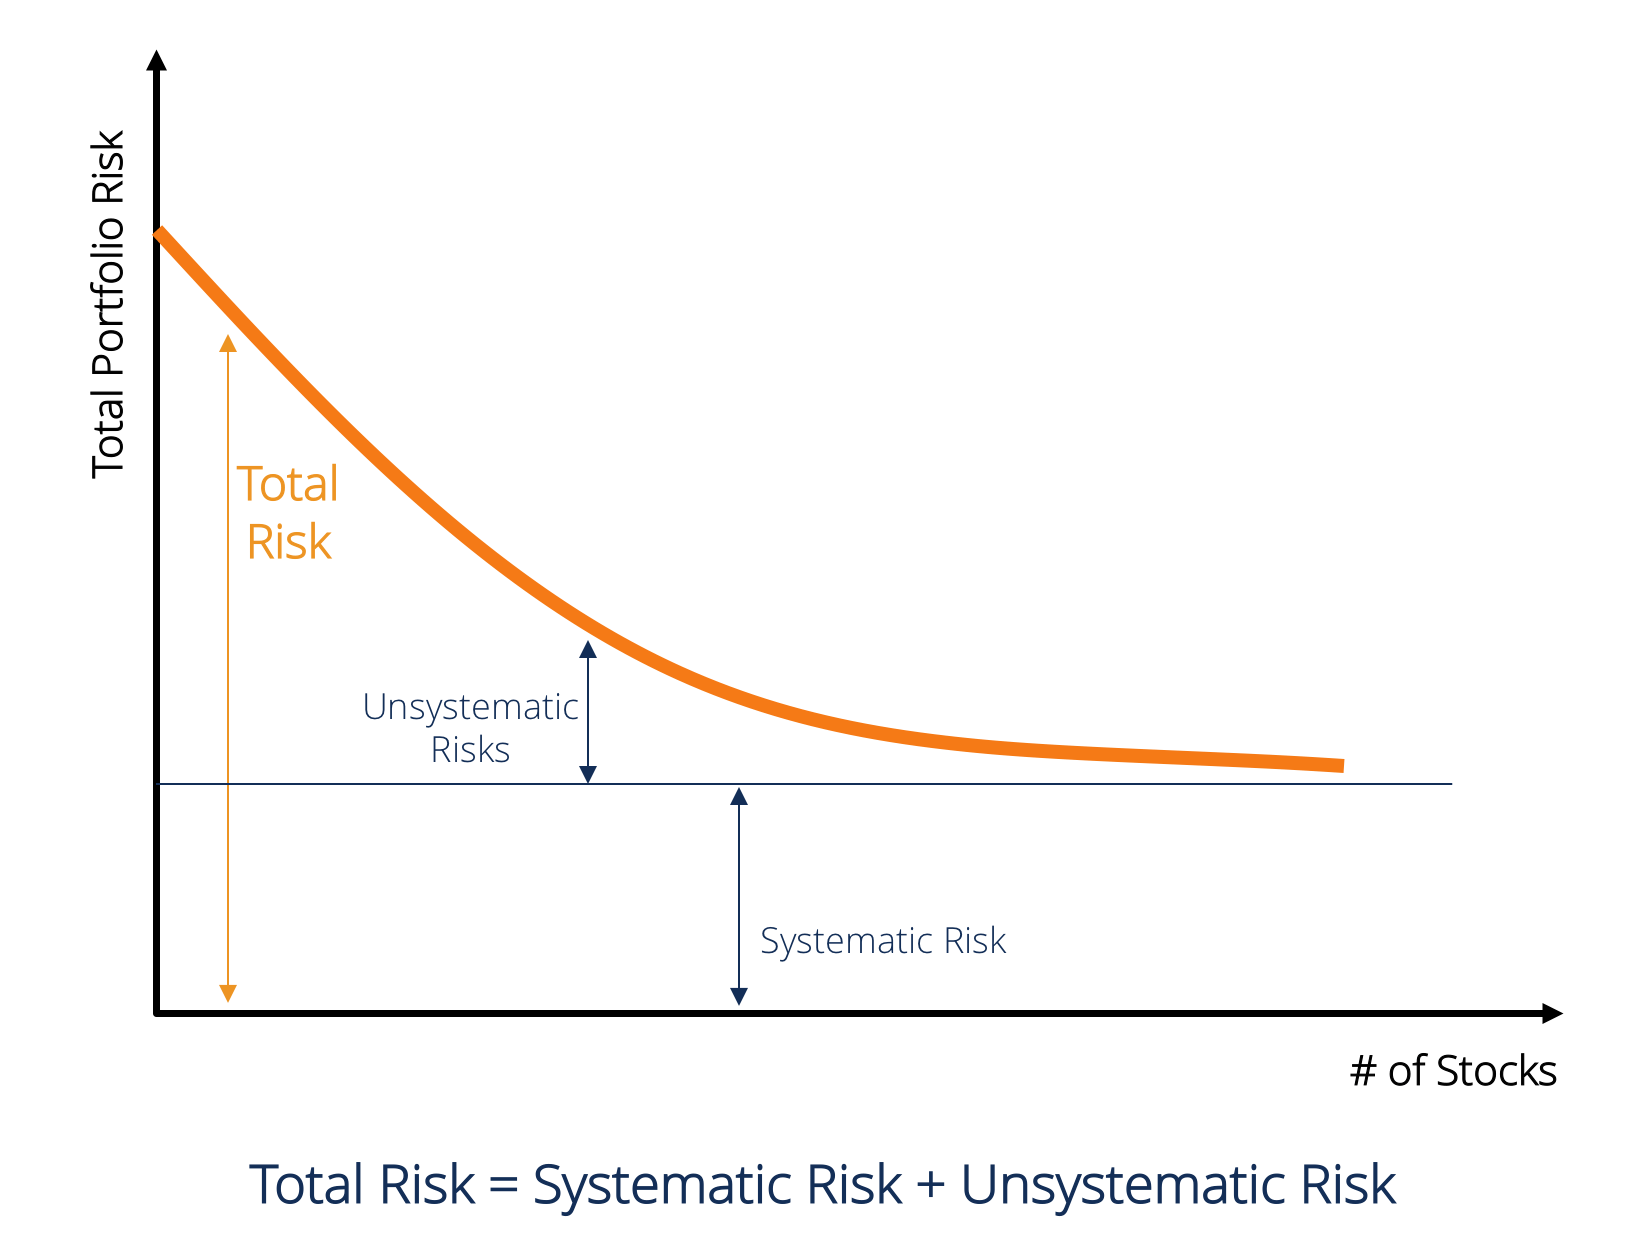
\includegraphics[width=\textwidth]{images/totalrisk.png}
\end{figure}

\paragraph{Unsystematic Risk} Is the risk specific to a company or industry. It is also known as diversifiable risk. It can be reduced through diversification.
\paragraph{Systematic Risk} Is the risk specific to the entire market. Also known as undiversifiable risk, affecting the overall market.


\begin{itemize}
    \item The benefit of diversification varies over time.
    \begin{itemize}
        \item Correlation among assets might change;
        \item Diversification does not protect against a generalized decrease in returns and increase in risk.
    \end{itemize}
    \item When all assets move together, like during a financial crisis, diversification benefits shrink.
    \begin{itemize}
        \item Hedging against risk becomes more difficult.
    \end{itemize}
\end{itemize}

\subsection{The Emergence of Modern Portfolio Theory}
\begin{itemize}
    \item The concept and intuition of the benefit of diversification has been around for a long time.
    \item However, its modern concept is theorized more recently.
    \item The main conclusion is that: \textbf{investors should not only hold portfolios but also focus on the correlation among the securities included.}
\end{itemize}

\section{Efficient Portfolio Frontier}
\subsection{Investment Opportunity Set}
Include as many assets as possible, from different sectors.
\subsection{Minimum Variance Frontier}
\begin{itemize} 
    \item We create a portfolio of assets;
    \item We are interested in pushing the frontier onto the north-west: 
    \begin{itemize}
        \item Minimizing the variance for a given return.
    \end{itemize}
    \item We calculate the combinations with different weights that minimize the variance for a given return.
    \item If we combine all the available assets and select the weights giving the lower variance for a given return, we end up with the \textbf{minimum variance frontier}.
    \item All portfolios on this frontier display a lower variance and a higher return than any individual asset.
\end{itemize}
\paragraph{Note:} The frontier uses all the available assets.
An efficient portfolio is \textit{any} portfolio on the minimum variance frontier.

\section{The Efficient Portfolio}
\subsection{Risk-free Asset}
\begin{itemize}
    \item To select the most efficient portfolio on the frontier, we need to add a risk-free asset.
    \item A risk-free asset will allow us to:
    \begin{itemize}
        \item Find the most efficient portfolio;
        \item Draw the capital allocation line (CAL);
        \item Create any risk-return combination for investors.
    \end{itemize}
    \item The efficient \textbf{investor portfolio} will always be a \textbf{combination} of:
    \begin{itemize}
        \item The risk-free asset;
        \item The efficient portfolio.
    \end{itemize}
\end{itemize}

\section{Capital Allocation Line}
\begin{itemize}
    \item A capital allocation line is a line that allocates capital between two assets;
    \item We will allocate between a risk-free and a risky asset;
    \item We will still think in terms of risk and return trade-off;
    \item We need two elements: an \textbf{intercept}, and a \textbf{slope}.
\end{itemize}
\subsection{A Risk-free Asset}
In our case, assume a portfolio of two assets, a risk-free asset and a risky asset. Expected return can be determined as:
\[E(R_p) = W_1R_f + (1-W_1)E(R_i)\]
Because the risk-free asset has 0 risk, its variance is equal to zero, hence, the variance of this portfolio can be calculated as:
\[\sigma_p{^2} = (1-W_1)^2\sigma_i{^2}\]
And volatility:
\[\sigma_p = \sqrt{(1-W_1)^2\sigma_i{^2}} = (1-W_1)\sigma_i \]
If we combine the portfolio return and standard deviation formula, we can rewrite the expected return in terms of risk.
\\ The expected return of a portfolio that mixes a risk-free asset and the optimal portfolio is based on two elements:
\[E[R_p] = R_f + \frac{E(R_i) - R_f}{\sigma_i}\sigma_i\]
\begin{itemize}
    \item The risk-free rate: $R_f$
    \begin{itemize}
        \item It is the Y-intercept;
        \item You cannot earn less than that.
    \end{itemize}
    \item The market price of risk: $\frac{E(R_i)-R_f}{\sigma_i}\sigma_p$
    \begin{itemize}
        \item It is the slope of the capital allocation line (CAL);
        \item The highest, the best: plus it is high, plus the risk is profitable.
    \end{itemize}
\end{itemize}
\subsection{The Capital Allocation Line (CAL)}
\begin{itemize}
    \item The combination between a risky asset and a risk-free asset is called the \textbf{capital allocation line};
    \item The risk-free rate does not change;
    \item Maximizing this angle maximizes your benefits for the risk you are taking.
    \item You do not control the market price of risk;
    \begin{itemize}
        \item It is priced by the market.
    \end{itemize}
    \item At an investor level, you can vary your risk, by changing your weights in the portfolio.
\end{itemize}
\subsection{CAL and Optimal Portfolio}
\begin{itemize}
    \item Using the CAL, we will now find \textbf{the} optimal portfolio;
    \item It is one of the portfolios on the efficient frontier;
    \item By using the risk-free asset, you maximize your risk-return ration.
    \item Mathematically, it is the point that is tangent between the efficient frontier and the CAL.
    \item You cannot achieve a point better than one on the CAL;
    \begin{itemize}
        \item This would only be by changing the set of assets.
    \end{itemize}
    \item By holding a risk-free asset, an investor can achieve a point of higher return than the Markowitz Efficient Frontier with the same risk-level.
    \begin{itemize}
        \item Negative weight on the risk-free asset (Y).
    \end{itemize}
    \item The CAL and the optimum portfolio evolve over time.
    \begin{itemize}
        \item If the risk-free asset return changes, it will affect the CAL Y-intercept;
        \item Hence, it will modify the CAL, and which portfolio is optimum.
    \end{itemize}
\end{itemize}
\begin{figure}[h]
    \centering
    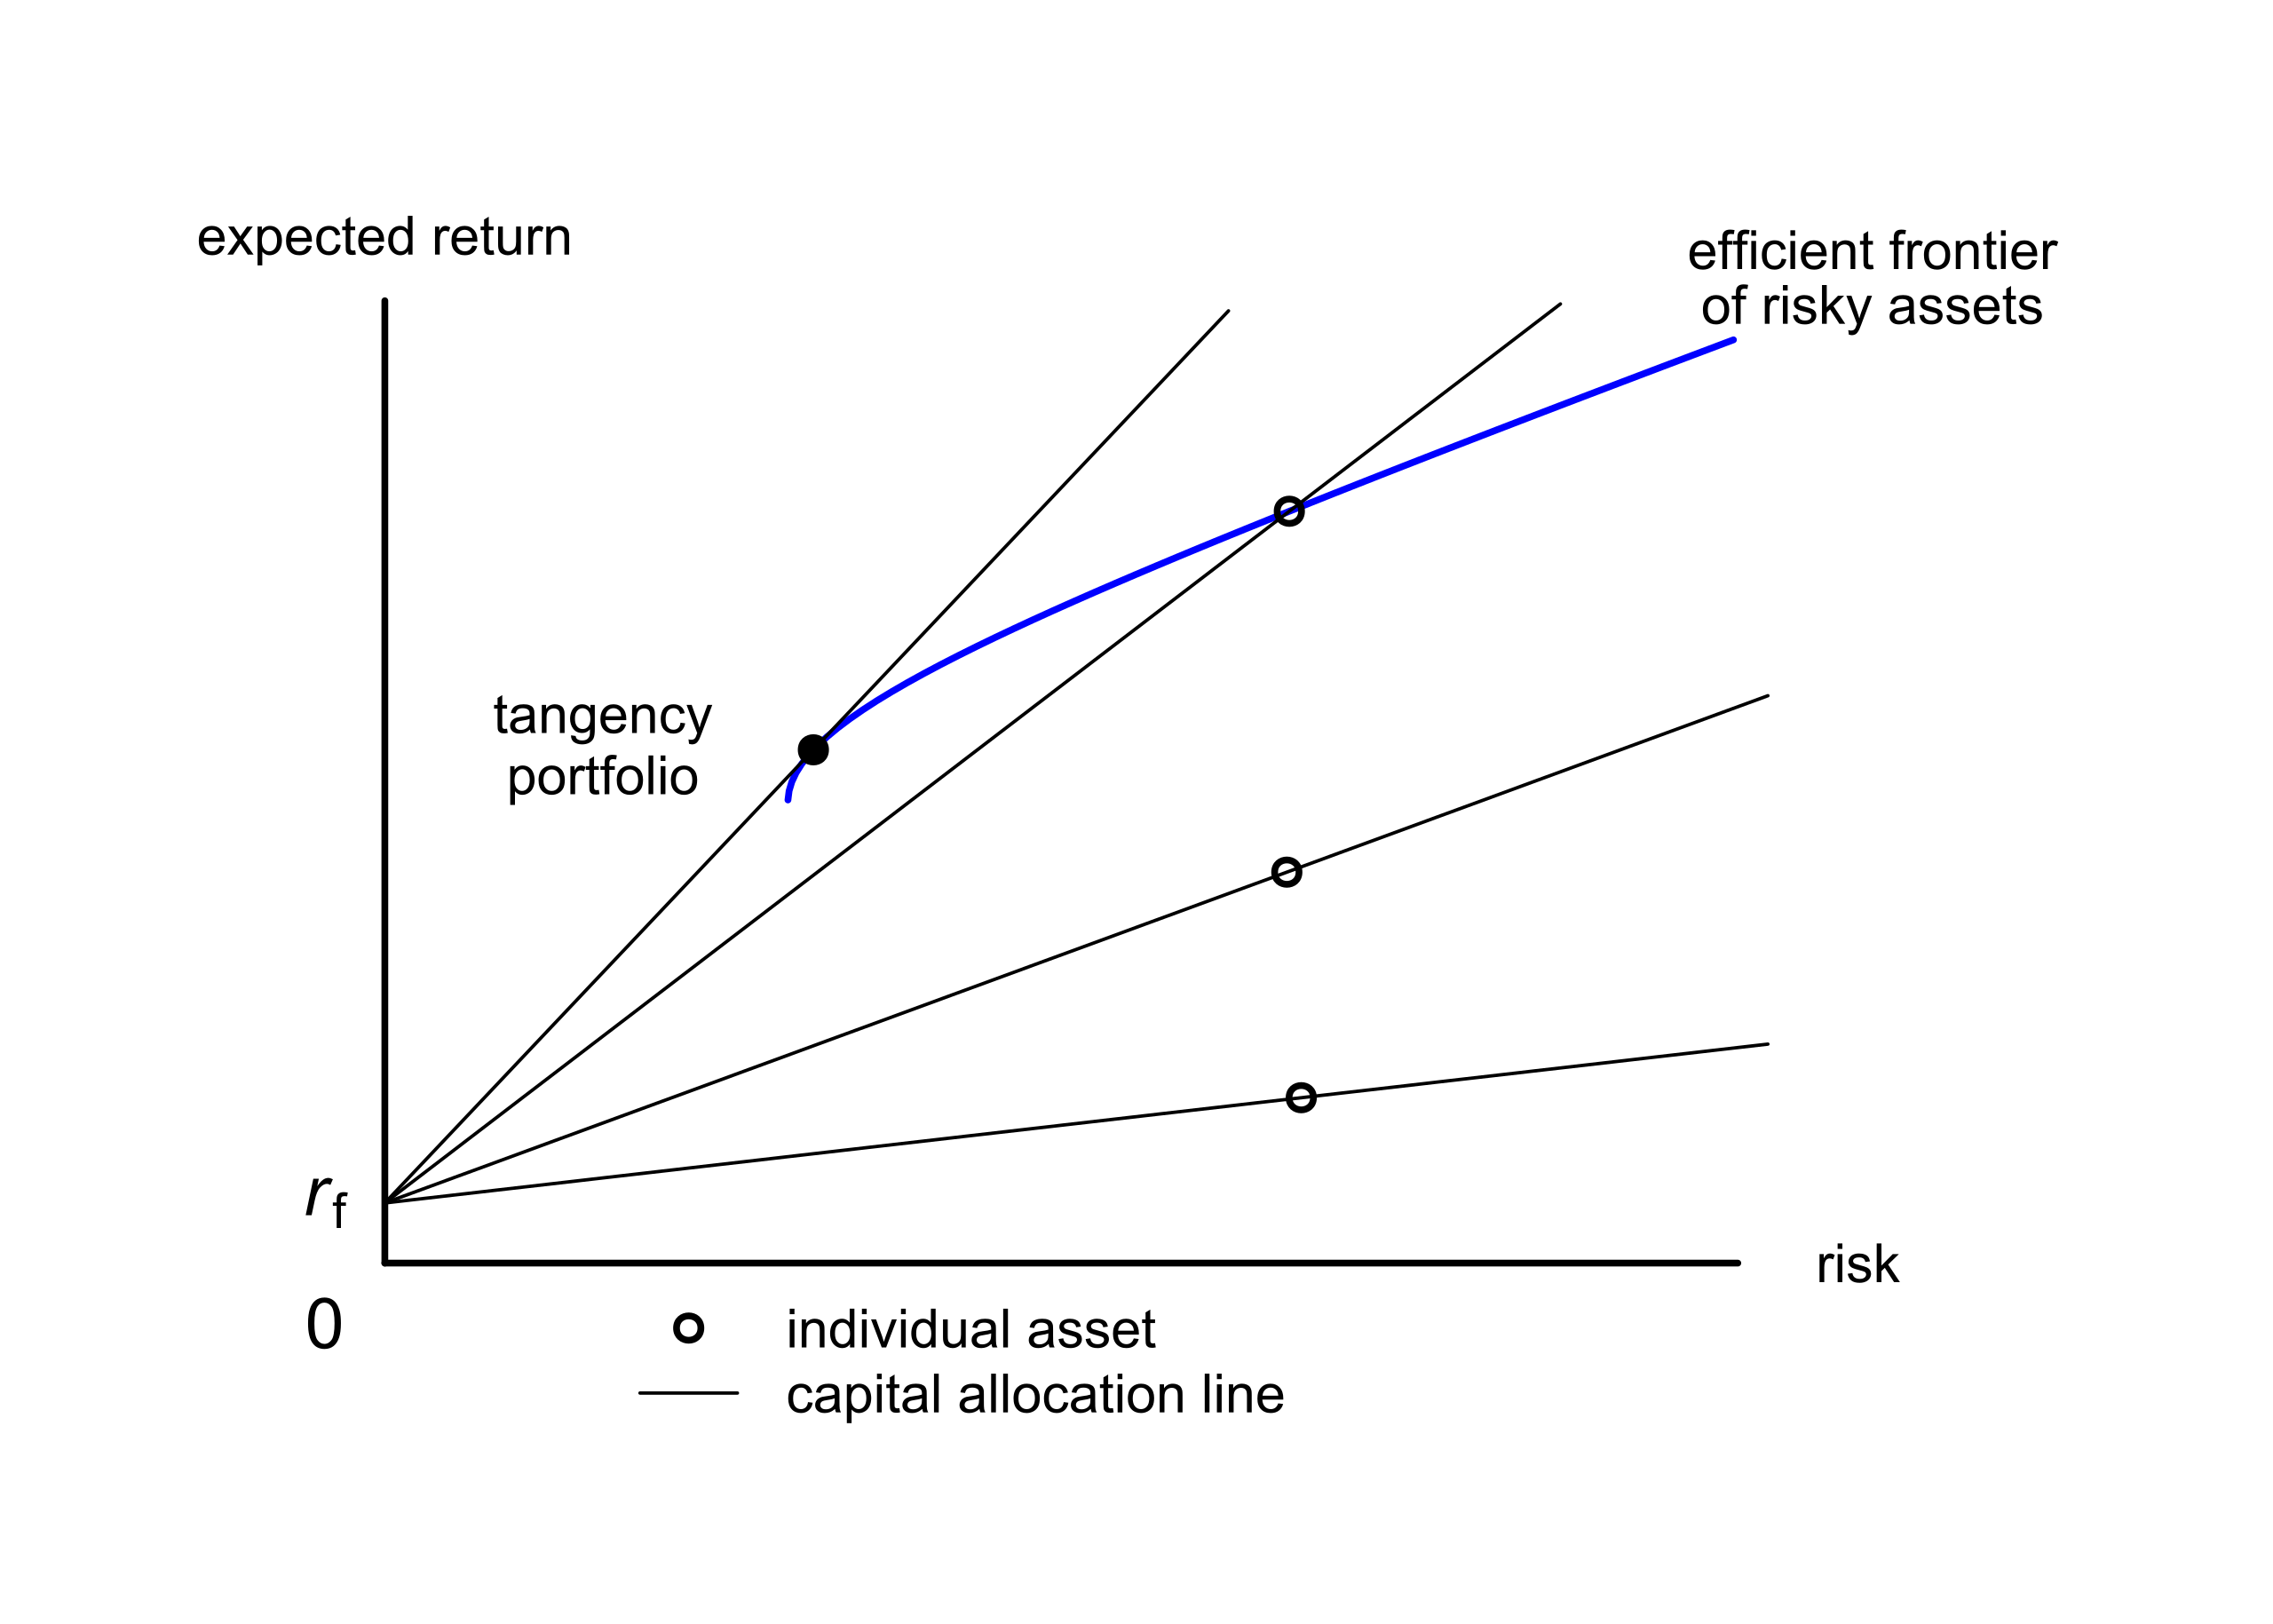
\includegraphics[width=\textwidth]{images/cap.png}
\end{figure}

\section{Optimal Investor Portfolio}
All investors will choose a \textbf{combination} of the risk-free and optimum portfolio. They will just change their weightings. But how do we know which portfolio will be chosen by a \textbf{specific investor}?
\subsection{The concept of Risk Aversion}
The choice of portfolio will differ across individuals because each individual has a different risk aversion.
\begin{itemize}
    \item Risk-seeking: utility increase with uncertainty.
    \begin{itemize}
        \item The individual will preferred a gamble with an expected value of £45 than a certain £50;
        \item Lottery and casinos.
    \end{itemize}
    \item Risk-neutral
    \begin{itemize}
        \item The individual is indifferent between the gamble or a £50 guaranteed income;
        \item A billionaire may be indifferent in this case.
    \end{itemize}
    \item Risk-adverse
    \begin{itemize}
        \item The investor will prefer a certain value of £50 than an expected value of £45;
        \item The risk-return trade-off is an indicator of risk-aversion;
        \item Historical data supports risk-aversion: higher returns, come with higher risks.
    \end{itemize}
\end{itemize}

\subsection{Utility Theory}
\begin{itemize}
    \item The \textbf{utility} he derives from the guaranteed income of £50 greater than the \textbf{utility} he derives from the alternative.
    \item Individuals are different in their preferences.
    \begin{itemize}
        \item All risk-averse investors will not rank their investments in the same manner;
        \item With a guaranteed outcome of £40, some may find it inadequate.
    \end{itemize}
    \item We can calculate the utility of an investor.
    \item This is not its return: it combines return and risk.
    \begin{itemize}
        \item Utility is a function of return for each individual;
        \item Individuals prefer higher utility.
    \end{itemize}
    \item We usually assume that investors are adverse to risk.
    \item There are plenty of ways to \textbf{modelize} utility.
\end{itemize}
\paragraph{The formula} \[U = E(r) - \frac{1}{2}A\sigma^2\]
\begin{itemize}
    \item U = Utility of an investment;
    \item E(r) = Expected Return;
    \item A = Measure of risk tolerance or risk aversion - can be either negative or positive;
    \begin{itemize}
        \item Risk adverse investor: $A>0$
        \item Risk neutral investor: $A=0$
        \item Risk seeking investor: $A<0$
    \end{itemize}
    \item $\sigma^2$ = Variance or risk.
    \item Higher returns = higher utility;
    \item Higher variance reduce/increase the utility, depending on A;
    \item A risk-free asset generates the same utility for all individuals.
\end{itemize}

\section{Indifference Curve}
An indifference curve plots the combination of risk-return pairs that an investor would accept to maintain a given level of utility. For each investor there is an infinity of indifference curves, but each indifference curve for each investor never cross over each other.
\begin{itemize}
    \item Represent the trade-off between risk and returns, with the \textit{same utility}.
    \item All risk-adverse investors will prefer curves on the north-west.
    \item Risk-adverse curves are convex because as risk increases, an investor needs even higher returns to compensate.
    \item The \textbf{slope} of curves is the \textbf{same for one investor} and different among investors.
\end{itemize}
\begin{figure}[h]
    \centering
    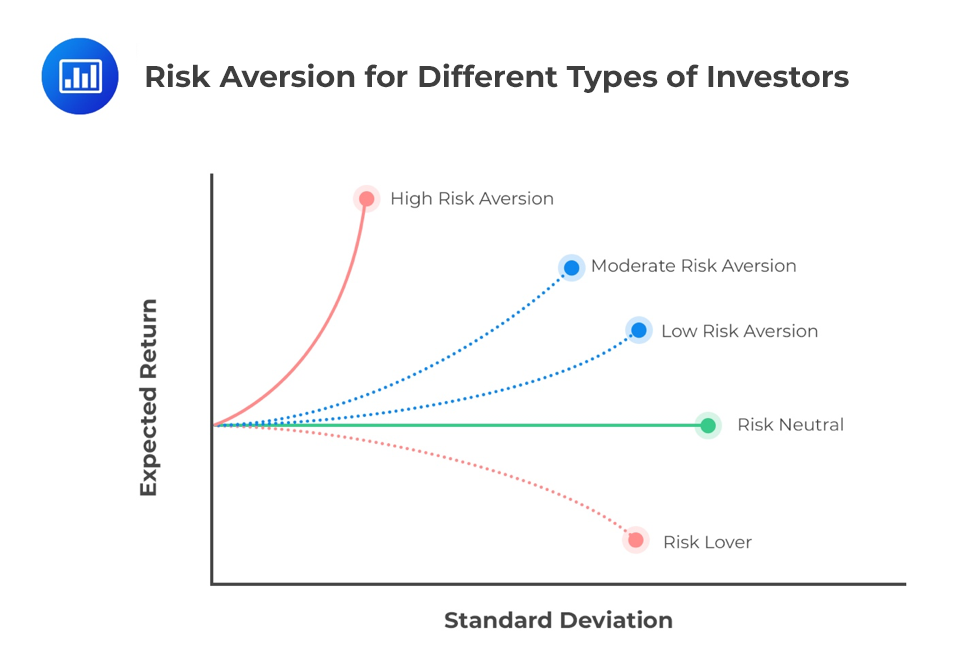
\includegraphics[width=\textwidth]{images/Risk-Aversion-for-Different-Types-of-Investors.png}
\end{figure}

\section{Optimal Investor Portfolio}
\begin{itemize}
    \item To know which combination is optimal for a given investor, we will use its indifference curve.
    \item The optimal investor's portfolio is the one which is tangent with the indifference curve.
    \begin{itemize}
        \item It gives them the highest \textbf{achievable} return.
        \item Lower or higher curbs, respectively, give:
        \begin{itemize}
            \item A lower utility;
            \item An unachievable utility.
        \end{itemize}
    \end{itemize}
    \item There is a different optimal portfolio for each investor - depending on its risk-aversion.
    \begin{itemize}
        \item All the points on CAL(P) are achievable;
        \item The selection will depend on the investor's preference.
    \end{itemize}
\end{itemize}
\section{The Two-Fund Separation Theorem}
\begin{itemize}
    \item Efficient Frontier;
    \item The Capital Allocation Line;
    \item Indifference Curve;
\end{itemize}
These concepts can be synthesized as a key theorem of modern portfolio theory.
\begin{itemize}
    \item \textbf{The two-fund separation theorem:} we can divide an investor's problem into two distinct steps.
    \begin{itemize}
        \item The investment decision;
        \item The financing decision.
    \end{itemize}
    \item \underline{For the investment decision:} all investors, regardless of taste, risk preferences and initial wealth, will hold a combination of two funds:
    \begin{itemize}
        \item A risk-free asset;
        \item The optimal portfolio of risky assets.
    \end{itemize}
    \item \textbf{Note:} All investors should lie on CAL(P).
    \item \underbar{For the financing decision:} each investor chooses the appropriate weight of risk-free and risky portfolio (P).
    \item The utility indifference curve of each investor will determine the investor's allocation to risky assets.
    \begin{itemize}
        \item Portfolios before the optimal risky portfolio are obtained by lending at the risk-free rate.
        \item Portfolios beyond the optimal risky portfolio are obtained by borrowing at the risk-free rate.
    \end{itemize}
\end{itemize}
\section{Summary of the Optimal Portfolio Choice}
\begin{itemize}
    \item Build the minimum variance frontier using all the assets available;
    \item Calculate and draw the capital allocation line (P) that is tangent to the minimum variance frontier.
    \item Use the investor's utility curves to obtain the portfolio that lies on the utility curve and on the capital allocation line (P).
\end{itemize}

\end{document}